\pdfbookmark[section]{Exempt Delegations}{Exempt Delegations}
\section{Exempt Delegations}

Exempt delegations (proposed in LSM~\cite{liquidity-staking-module})
are a mechanism to alleviate the Principal--Agent problem in liquid staking.
An exempt delegation amount $c$, measured in \asset, is associated
with each validator. It is a measure of the validator's trustworthiness.
The liquid staking protocol is now redesigned to impose restrictions
on how much of the protocol's pooled moneys can be delegated to a particular
validator based on the validator's exempt delegation.
The restriction is
parameterized by a factor $\phi$ (in practice, $\phi > 1$)
and is given by the inequality $b \leq \phi c$: Only up to $b$ \assets
are allowed to be delegated by the liquid staking protocol
to a validator with $c$ \assets in exempt delegations.

A new validator begins its lifecycle with $c = 0$. They can then
raise their own exempt delegation amount by locking aside a
chosen amount of \asset, and marking it as \emph{exempt}. Those
assets are delegated to the validator as usual. However,
the \emph{exempt}
marking means that those delegated assets cannot be part of the liquid
staking protocol pool, but must remain locked aside. Additionally,
these specially marked delegations are slashed\footnote{We abstract some
of the irrelevant implementation details here. See Appendix~\ref{sec:lsm}
for how the real protocol works in the context of Cosmos.}
at a potentially higher rate $q \geq p$. Exempt delegated assets cannot
be undelegated in a way that would cause a violation of the inequality
$b \leq \phi c$.

Principals, whether wise or unwise, do not participate in exempt
delegations; instead, it is the validator who exempt delegates to
themselves (or someone who trusts the validator for extrinsic reasons).
This means that, in case of validator misbehavior, the exempt delegation
slashing $qc$ is a penalty that only affects the validator.

\import{./}{exempt-delegation-attack-diagram.tex}

This raises
the cost of the attack described in the previous section. The
adversary must first, at time $t_1$ (where $t_0 < t_1 < t_2$), exempt delegate a sufficient amount
$c \geq \frac{b}{\phi}$ \asset to $\mathcal{V}$ before she can liquid stake $b$ \asset.
Whereas the \stassets
corresponding to those $b$ \assets can be, as before, sold at $t_3$ to
separate the agent from the principal, the $c$ amount remains with the
agent, holding her financially liable to misbehavior. After equivocation at $t_4$,
in addition to any other costs, the adversary loses $qc$ \asset. At the conclusion
of the attack, the adversary undelegates the unslashed $(1 - q)c$ exempt delegation.
The timeline of the attack is illustrated in Figure~\ref{fig:exempt-timeline}
(the flash loan indication is explained when we introduce the cost of borrowing).

The attack may remain profitable despite exempt delegations.
The rational adversary should not waste any unnecessary resources on
$c$; therefore, she can set $c = \frac{b}{\phi}$. The profit of the attack now
becomes $b^* - b' - \frac{q}{\phi}b$.
The intuition for why exempt delegations protect the system is that,
for the adversary to profit from the short, she must cause a significant
shift in the price. The shift in the price is determined by the factor
$p\frac{b}{b_0}$, so the adversary aims for a large $b$. But because $b \leq \phi c$
must be respected, this incurs a large penalty $qc = \frac{q}{\phi}b$.

\noindent
\textbf{The cost of borrowing.}
So far, we have allowed the adversary to take a loan indiscriminately without
any concern for collateral. In practice, loan platforms
require a collateral, so the attack impact will be limited by the adversary's
initial capital. Let $u$ \asset be the initial capital of the adversary, and
let $\gammastasset$ be the collateral ratio of a standard \stasset
loan. The adversary uses the whole initial capital of $u$ \asset as
collateral to obtain a loan of $z = \frac{u}{\gammastasset} \frac{s_0}{b_0}$ \stasset.
The loaned $z$ \stasset are converted to $b^*=\frac{u}{\gammastasset}$ \asset
and utilized by the adversary in the next steps of the attack.

It was also previously assumed that the adversary has $c$ \asset to exempt
delegate ($t_1$) and $b$ \asset to deposit in the protocol ($t_2$) at her disposal.
Instead of requiring these as extra assets set aside, we will make them part of
the loan obtained by the adversary. That way, all the initial capital of
the adversary can be used to maximize her shorting leverage.

Notice that the adversary deposits $b$ \asset in the protocol at $t_2$ and
gets them back at $t_3$ after selling the \stasset obtained from the deposit.
These two actions can be performed in a single transaction. Hence, a flash
loan can be used to obtain the required $b$ \asset at $t_2$ and be repaid,
including a $\betaasset b$ \asset flash loan cost, at $t_3$, after the adversary gets
$b$ \asset back.
The flash loan is illustrated in Figure~\ref{fig:exempt-timeline}.

To perform the attack, part of the $b^*$ funds are used to exempt delegate
$c = \frac{b}{\phi}$ \asset to $\mathcal{V}$ at $t_1$, and another part
to pay $\betaasset b$ \asset for the flash loan cost at $t_3$.
Hence $c + \betaasset b \leq b^*$ and the adversary may use up to
$b \leq \frac{u}{(\frac{1}{\phi} + \betaasset)\gammastasset}$
to move the price.

Taking into consideration the flash loan cost as well, the final profit of the attack is now
$\alpha = b^* - b' - qc - \betaasset b$.
Solving for $\frac{d\alpha}{db} = 0$ gives the optimal $b = \sqrt{\frac{u f p b_0}{(\betaasset + \frac{q}{\phi})\gammastasset}} - b_0$,
which maximizes
the adversary's profit, subject to the constraints
$0 \leq b \leq \frac{u}{(\frac{1}{\phi} + \betaasset) \gammastasset}$.
In non-extreme market conditions, if the attack is profitable, the bound
$b \leq \frac{u}{(\frac{1}{\phi} + \betaasset)\gammastasset}$ will not be reached,
and the adversary will use the value
$b = \sqrt{\frac{u f p b_0}{(\betaasset + \frac{q}{\phi})\gammastasset}} - b_0$.
%TODO(w/ dionyziz, probably e-print): This is probably true, maybe present plot with optimal b values

What would it take to disincentivize the adversary from attacking the protocol?
As protocol designers, we need to carefully parametrize the liquid staking protocol
to ensure the adversarial profit is not positive. This will render the attack irrational
and the protocol secure in the rational model. To achieve this, we must select
the parameter $\frac{\phi}{q}$ in a way that $\alpha \leq 0$.
Plugging in the optimal value for $b$ in the inequality $\alpha \leq 0$ and solving
the resulting equation for $\frac{\phi}{q}$ yields

% (-b0*β*γ - 2*sqrt(f)*sqrt(p)*u*sqrt(f - 1) + f*p*u + f*u - u)/(b0*γ)
% (1/(b0*γ)) * (f*p*u + f*u - b0*β*γ - 2*u*sqrt(fp*(f-1)) - u)
\begin{gather*}
  \frac{\phi}{q} \leq \frac{b_0 \gammastasset}{f p u + f u - b_0 \betaasset \gammastasset - 2 u \sqrt{fp (f-1)} - u}\,. \label{eq:phi-choice} \tag{$\ast$}
\end{gather*}

Plugging the appropriate values
into $p$, $\betaasset$, $f$, $b_0$, $\gammastasset$ and $u$
designating the conditions the protocol
operates under, the protocol designers can calculate a secure value
$\frac{\phi}{q}$.
A higher exempt delegation slashing rate $q$ makes the attack more expensive. This
is because a larger portion of the exempt delegation $c$, holding the adversary accountable,
is slashed. A lower exempt delegation factor $\phi$ also makes the attack more expensive
since a larger exempt delegation is required to liquid stake the same $b$ \asset.
Hence, a lower $\frac{\phi}{q}$ makes the protocol less vulnerable to the attack.
We recommend always setting $q = 1$ if possible, as this allows for
larger values of $\phi$, increasing liquidity, without any harm to anyone
besides the adversary.

The cost of borrowing money increases when the collateral ratio
$\gammastasset$, the flash loan cost factor $\betaasset$ or the loan cost factor $f$
increase. While the cost of borrowing money goes up, the attack becomes less profitable
for the adversary. Thus, the protocol can afford to increase $\frac{\phi}{q}$
and still remain secure. This is illustrated in
Figure~\ref{fig:plotf} for an adversary with $30\%$ market domination $\frac{u}{b0}$,
and an adversary with $50\%$ market domination $\frac{u}{b0}$.
While $f$ increases, the safe parameter $\frac{\phi}{q}$ can increase with it.
The black line indicates where the attack becomes unprofitable for the adversary ($\alpha = 0$).
The white area under the black line represents the configuration in which
the protocol is secure in the rational model.

As an illustration,
we consider a blockchain with slashing percentage
$p = 0.5$ and market conditions\footnote{Lido stETH borrowing rates
on Aave~\cite{aave} as of 27 Jan, 2023.}
with \asset flash loan cost factor $\betaasset = 0.0009$ and
collateral ratio $\gammastasset = 146\%$.
In Figure~\ref{fig:plotf} we plot the dependencies between $f$ and adversarial
profit. At the time of writing, if the attack duration is $20$ sec, we have
$f = 1 + 10^{-8}$.

%TODO (tzinas and w/dionyziz): find out if setting $b_0$ here is necessary
%, a liquid staking protocol with $b_0 = 10000$ \asset initial holdings,

\begin{figure}[htb]
  \centering
  \begin{subfigure}{0.49\textwidth}
    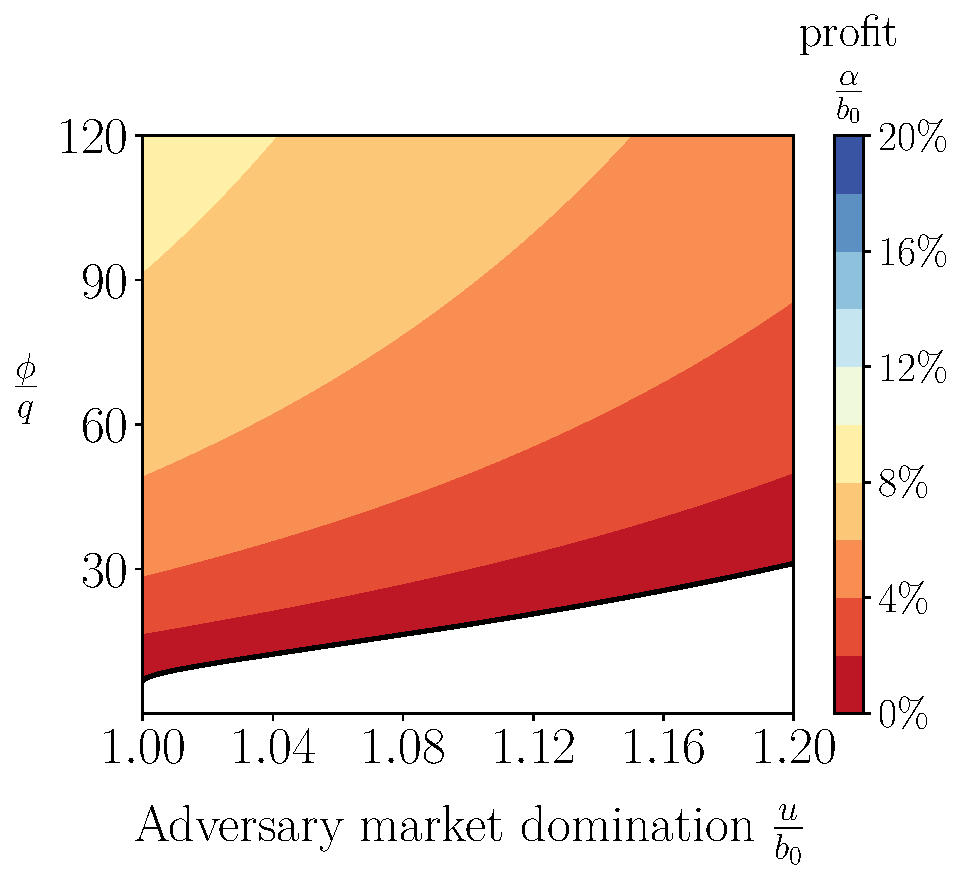
\includegraphics[width=\textwidth]{./plots/plotf30.pdf}
    \caption{Collateral $u$ is $30\%$ of $b_0$.}
    \label{fig:plotf30}
  \end{subfigure}
  \hfill
  \begin{subfigure}{0.49\textwidth}
    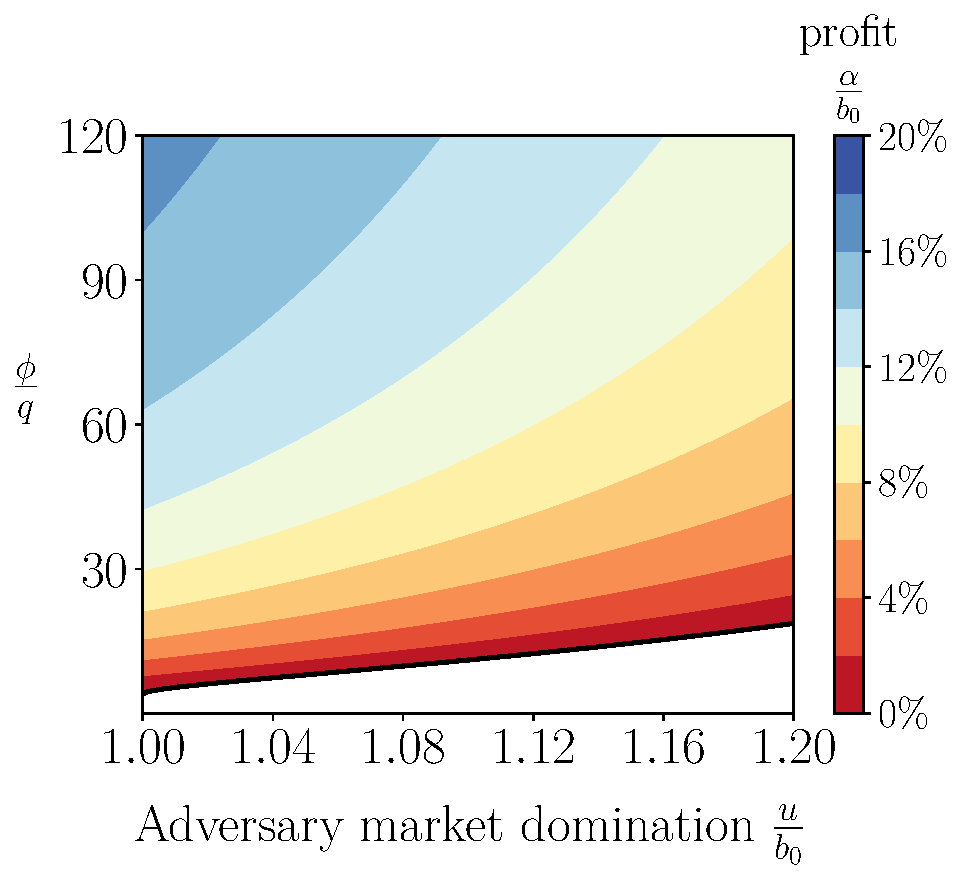
\includegraphics[width=\textwidth]{./plots/plotf50.pdf}
    \caption{Collateral $u$ is $50\%$ of $b_0$.}
    \label{fig:plotf50}
  \end{subfigure}
  \caption{Cost of borrowing and attack profitability.}
  \label{fig:plotf}
\end{figure}


\noindent
\textbf{Free money borrowing.}
We saw that, in practice, $f \simeq 1$, and money borrowing is almost free
for short durations. Free money borrowing makes the adversary more powerful
and her attack more profitable.
Hence, if a parameter $\frac{\phi}{q}$ keeps the protocol secure when money
borrowing is free ($f = 1$, $\betaasset = 0$, $\gammastasset = 1$),
the same parameter $\frac{\phi}{q}$ keeps the protocol secure even when
money borrowing is not free. This is illustrated in
Figure~\ref{fig:compare-f-plotu}. Safe values of parameter $\frac{\phi}{q}$
for $f = 1$, indicated by the black line, are also safe for $f > 1$
under any adversarial market domination $\frac{u}{b_0}$.

%TODO (tzinas): check if the same happens for β and γ
% updated: happens for β, γ needs to be checked as well
%TODO (w/ dionyziz): where should we include the plots?

\begin{figure}[htb]
  \centering
  \begin{subfigure}{0.48\textwidth}
    \raisebox{3.7mm}{
    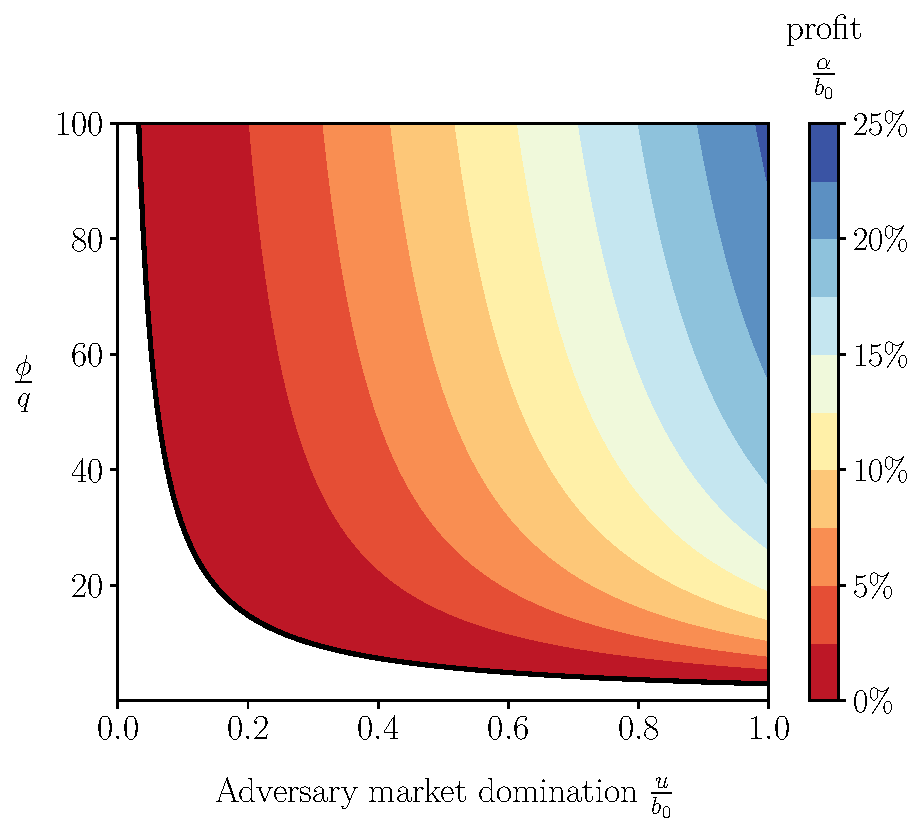
\includegraphics[width=\textwidth]{./plots/plotu.pdf}
    }
    \caption{Adversarial market domination and attack profitability
             for varying $\frac{\phi}{q}$.}
    \label{fig:contour-plotu}
  \end{subfigure}
  \hfill
  \begin{subfigure}{0.5\textwidth}
    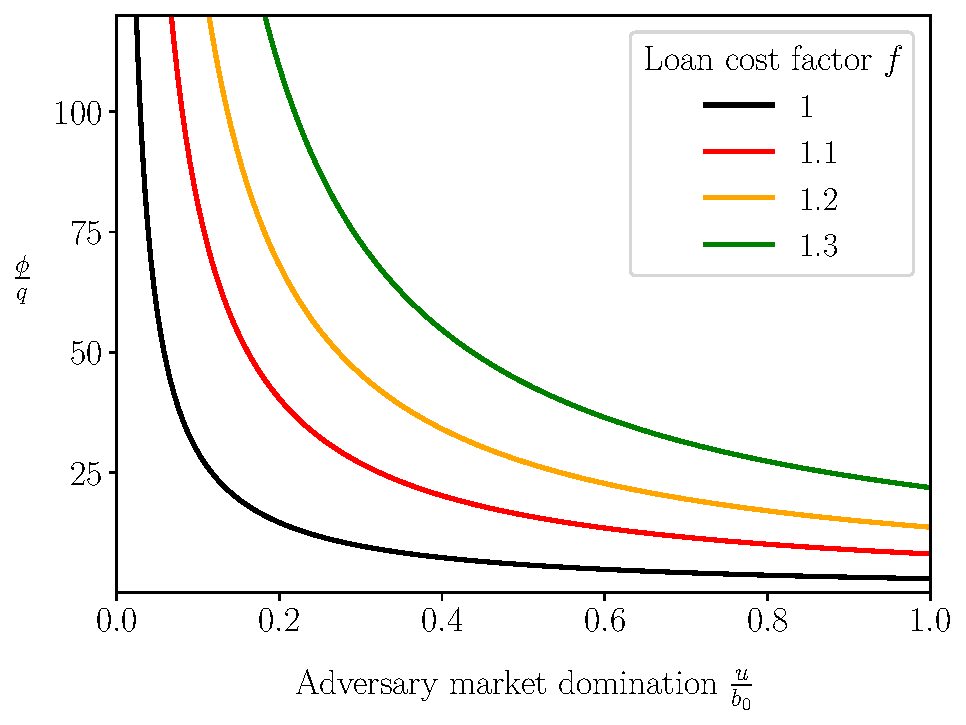
\includegraphics[width=\textwidth]{./plots/multiplef_plotu.pdf}
    \caption{Optimal $\frac{\phi}{q}$ system parametrizations
             for different adversarial market dominations $\frac{u}{b_0}$
             and market conditions $f$.}
    \label{fig:compare-f-plotu}
  \end{subfigure}
  \caption{Adversarial market domination and attack profitability.}
  \label{fig:plotu}
\end{figure}

Hence, we can greatly simplify the above calculations by assuming that money borrowing is free.
Concretely if flash loans are free ($\beta = 0$), interest rates are zero ($f = 1$),
and the collateral ratio is $\gamma = 100\%$, equation~\eqref{eq:phi-choice} simplifies to:
%TODO (w/ dionyziz): why not use \betaasset and \gammastasset?

\begin{gather*}
  \frac{\phi}{q} \leq \frac{b_0}{pu} \label{eq:phi-choice-simple}
\end{gather*}

This equation can be used in practice to calculate the appropriate value
of $\frac{\phi}{q}$ that can withstand an adversary with a market presence of $\frac{u}{b_0}$
(due to the very short duration of the attack, the cost of money borrowing does not alter
the final result by much). Note that, even though the attack might be profitable for a
large $p$, a lower value of $p$ may make the attack unprofitable.
Additionally, protocols with more liquidity $b_0$ are less prone to attack,
because a larger capital $u$ is required to achieve the required market domination
$\frac{u}{b_0}$.
For example, if the liquid staking protocol has $b_0 = 1000$ \asset in deposits,
and the adversary can use a capital of $u = 100$ \asset to attack the protocol
($\frac{u}{b_0} = 10\%$ market domination),
if $p = q = 100\%$ is the slashing rate, then $\phi \leq \frac{b_0}{u} = 10$
is a safe protocol parametrization. Attack profitability for different adversarial
market dominations $\frac{u}{b_0}$, assuming free money borrowing and $p = 50\%$,
are illustrated in Figure~\ref{fig:contour-plotu}.
The white area under the black line ($\alpha = 0$) consists of safe values
of the parameter $\frac{\phi}{q}$.

Proportional representation and fair punishment, as indicated in
Section~\ref{sec:attack}, are two conflicting properties in liquid
staking. An adversary can always leverage proportional
representation to cause the unfair punishment of principals.
However, with the introduction of exempt delegations and a carefully selected
$\frac{\phi}{q}$ parameter, a liquid staking protocol can achieve both of these
properties in the rational model.

\noindent
\textbf{Repeating the attack.} If the adversary finds herself in a situation
where the attack is profitable, the attack can be repeated in quick succession
to siphon off almost all of the money in the liquid staking protocol.
This corresponds to moving across the $x$ axis in Figure~\ref{fig:contour-plotu}.
As the attack repeats, $b_0$ decreases and $u$ increases as money moves from
the reserves of the staking protocol to the hands of the adversary.
We conclude that the protocol must be configured with enough margin
such that the conditions for the attack never emerge.

%\begin{align*}
%  &a = b^* - b' - qc - \betaasset b\\
%  &a = \frac{b_0}{s_0}z(1 - (1 - p\frac{b}{b_0 + b})((1 + \rstasset)^{\Delta_z} + \betastasset)) - \betaasset b - \frac{q}{\phi}b\\
%  &a = \frac{u}{\gammastasset}(1 - (1 - p\frac{b}{b_0 + b})((1 + \rstasset)^{\Delta_z} + \betastasset)) - \betaasset b - \frac{q}{\phi}b\\
%\end{align*}
%
%Let $f = (1 + \rstasset)^{\Delta_z} + \betastasset$:
%
%\begin{align*}
%  &a = \frac{u}{\gammastasset}(1 - (1 - p\frac{b}{b_0 + b})f) - \betaasset b - \frac{q}{\phi}b\\
%\end{align*}

%\begin{gather*}
%  \frac{da}{db} = 0\\
%  \frac{u f p}{\gammastasset} \frac{b_0}{(b_0 + b)^2} - \betaasset - \frac{q}{\phi} = 0\\
%  \frac{u f p b_0}{\gammastasset (b_0 + b)^2} = \betaasset + \frac{q}{\phi}\\
%  \frac{u f p b_0}{\gammastasset (\betaasset + \frac{q}{\phi})} = (b_0 + b)^2\\
%  (b_0 + b)^2 - \frac{u f p b_0}{\gammastasset (\betaasset + \frac{q}{\phi})} = 0\\
%  b^2 + 2b_0b + b_0^2 - \frac{u f p b_0}{\gammastasset (\betaasset + \frac{q}{\phi})} = 0\\
%\end{gather*}